\chapter{Попередні роботи присвячені задачі стереобачення}

В першому розділі надано стислий огляд досліджень,
що пов'язані із задачею стереобачення.
Проводиться аналіз та порівняння деяких існуючих методів розв'язання задачі.
Розбір попередніх робіт дає змогу виявити недоліки
існуючих рішень та чітко поставити задачу,
що розв'язується в другому та третьому розділах дисертації.

\section{Динамічне програмування}

Вважається, що камера не вносить радіальних спотворень,
а два зображення отримуються шляхом її ідеального зсуву по горизонталі,
тобто пікселям рядка $y$ лівого зображення
$L_y \; : \; \left\{ 1, \dotsc, w \right\} \to C$, де $w$~---~ширина зображення,
відповідають пікселі рядка $y$
правого зображення $R_y \; : \; \left\{ 1, \dotsc, w \right\} \to C$,
$y = \overline{1, h}$, $h$~---~висота зображення,
а $C = \left\{ 0, \dotsc, 255 \right\}$~---~множина,
що задає інтенсивності пікселів.
Вважається, що в кожен рядок лівого зображення проектується свій об'єкт,
тому вектори зсувів для всіх рядків можна знаходити окремо шляхом
мінімізації штрафної функції
\begin{equation}\label{eq:overview:energy}
    E \left(\pmb{d}, y \right)
    = \sum \limits_{x = 1}^{w}
        f_{\left( x, y \right)} \left( d \left( x \right) \right)
    + \sum \limits_{x = 1}^{w}
        g \left(d \left(x \right), d \left( x + 1 \right) \right),
\end{equation}
яка називається енергією,
де $\pmb{d}$~---~вектор зсувів для рядка з номером $y$,
кожен елемент якого може приймати значення з множини
$\left\{ 0, 1, \dotsc, M \right\}$,
$L_y \left( x \right)$~---~інтенсивність пікселя з координатами
$ \left(x, y \right)$ на лівому зображенні,
а $R_y \left( x \right)$~---~інтенсивність пікселя з координатами
$\left( x, y \right)$ на правому зображенні.
Штрафна функція включає штраф за негладкість карти зсувів $g$ (бінарні штрафи)
і невідповідність кольорів співставлених пікселів на двох зображеннях $f$
(унарні штрафи).
Унарні штрафи
$f_{\left( x, y \right)} \left( d \right) = f \left(
    L_y \left(x \right),
    R_y \left( x - d \right)
\right)$ залежать від значеннь
інтенсивностей відповідних пікселів на лівому та правому зображеннях,
бінарні штрафи $g$~---~від зсувів двох сусідніх по горизонталі пікселів.

Для кожного рядка зображення будується граф
(рис.~\ref{fig:dynamic:programming:graph}),
де кожен піксель $x$ рядка $y$ є об'єктом,
а вершини в об'єктах відповідають можливим зсувам $d \left(x \right)$.
Назвемо їх мітками.
Сусідніми вважаються лише ті об'єкти, які відповідають сусіднім пікселям
(у кожного пікселя є лівий і правий сусідні пікселі).
Вага мітки в об'єкті $x$, що відповідає зсуву $d \left(x \right)$,
задається значенням функції $f_{\left( x, y \right)} \left( d \right)$,
а вага дужки між двома сусідніми об'єктами $x$ і $x + 1$~---~значенням функції
$g \left( d \left(x \right), d \left( x + 1 \right) \right)$.
Методом динамічного програмування знаходится
такий вектор зсувів $\pmb{d}$ для кожного рядка $y$
одного з зображень стереопари,
що відповідає найкоротшому шляху на побудованому графі
\cite{overview:cox:dynamic}.

\begin{figure}[h]
  \centering
  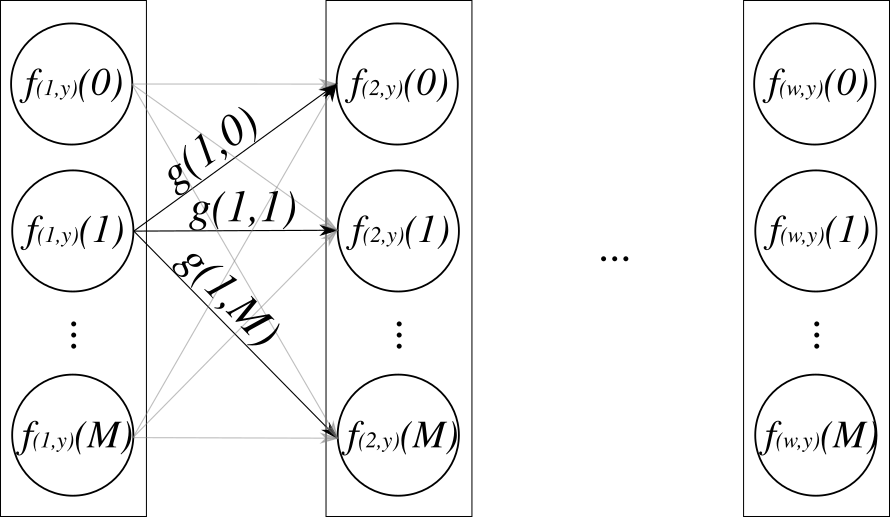
\includegraphics[width=0.8\textwidth]{images/dynamic_programming_graph}
  \caption{Граф, на якому розв'язується задача пошуку мінімального
           шляху методом динамічного програмування для пошуку вектора зсувів
           $\pmb{d}$ для рядка $y$ одного з зображень стереопари.
           Прямокутниками позначені об'єкти, окружностями~---~вершини,
           всередині яких зазначені штрафи, на стрілках зазначені штрафи,
           що накладаються на дужки між вершинами сусідніх об'єктів}
  \label{fig:dynamic:programming:graph}
\end{figure}

Недолiком методу динамiчного програмування є те, що вiн обробляє всi
рядки зображення незалежно, тобто не враховує узгодженості між рядками,
тому в простому випадку метод динамічного програмування не використовує
двовимірність задачі та не дає гладкої карти
глибин по вертикалі (рис. \ref{fig:overview:cox:dynamic}).

\begin{figure}[h]
  \centering
  \begin{subfigure}[b]{0.8\textwidth}
      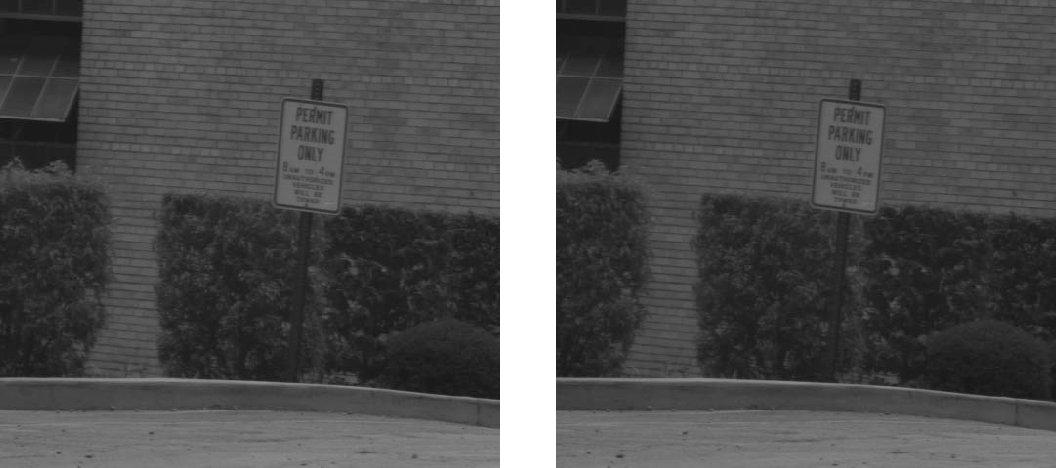
\includegraphics[width=\textwidth]{images/overview_cox_dynamic_left_right}
      \caption{Ліве та праве зображення}
  \end{subfigure}
  \begin{subfigure}[b]{0.4\textwidth}
      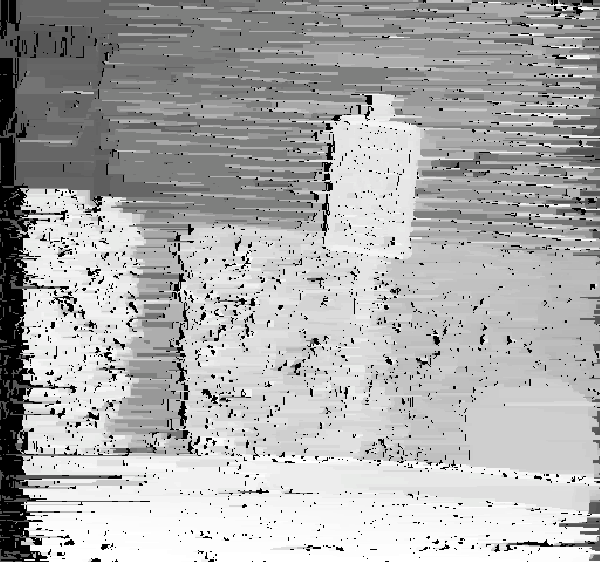
\includegraphics[width=\textwidth]{images/overview_cox_dynamic_result}
      \caption{Карта глибин}
  \end{subfigure}
  \caption{Результати, отримані методом динамічного програмування
           (зображення взяті зі статті \cite{overview:cox:dynamic})}
  \label{fig:overview:cox:dynamic}
\end{figure}

Водночас, алгоритм працює досить швидко,
а результати можна значно покращити (рис. \ref{fig:overview:wang:dynamic}),
наприклад розглядаючи вісім сусідів пікселя
замість двох та використовуючи сегментацію зображення за кольором
\cite{overview:wang:dynamic}.

\begin{figure}[h]
  \centering
  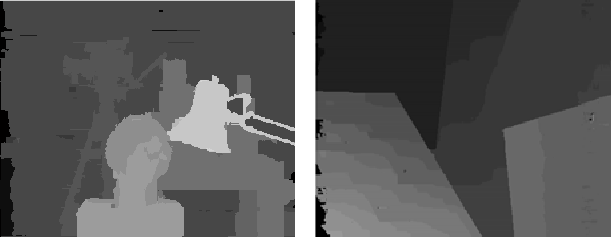
\includegraphics[width=0.8\textwidth]{images/overview_wang_dynamic}
  \caption{Результати, отримані за допомогою покращеного методу динамічного
           програмування
           (зображення взяті зі статті \cite{overview:wang:dynamic})}
  \label{fig:overview:wang:dynamic}
\end{figure}

\section{Нейронні мережі}

Нейронна мережа навчається на вхідних даних:
парах зображень та відповідній ним карті глибин.
Добре розмічені вхідні дані для навчання
наявні для зображень дороги.
Нейронна мережа, навчена на таких даних може давати погані результати для
зображень іншого середовища.
На рисунку \ref{fig:overview:luo:nn}
наведено приклад вхідних даних і результуючої карти глибин,
що була навчена за допомогою даних з набору <<KITTI Stereo>>
\cite{overview:geiger:nn}.

\begin{figure}[h]
  \centering
  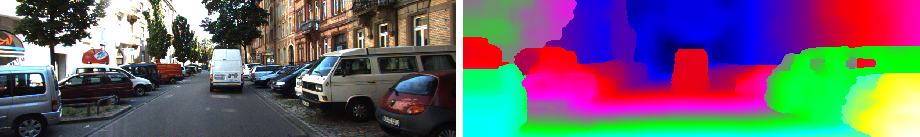
\includegraphics[width=\textwidth]{images/overview_luo_nn}
  \caption{Ліве зображення та карта глибин,
           отримана за допомогою нейронної мережі
           (зображення взяті зі статті \cite{overview:luo:nn})}
  \label{fig:overview:luo:nn}
\end{figure}

\section{Знаходження мінімального розрізу графа}

Задачею є мінімазація енергії \ref{eq:overview:energy}.
Будується граф-решітка, у якому вершинами є всі пікселі зображення.
Назвемо ці вершини основними.
Ваги вершин і дуг задаються як в методі динамічного програмування.
До графа додається дві допоміжні вершнии: джерело та стік,
які поєднуються з кожними іншими вершинами графу.
Кожній основній вершині має бути поставлена у відповідність
мітка~---~значення зсуву координати пікселя по відношенню до цієї ж координати
на іншому зображенні зі стереопари.
Застосовується алгоритм $\alpha$-експансії:
спочатку фіксується якась мітка в кожній основній вершині.
Також випадковим чином обирається ще одна мітка (однакова для всіх вершин).
Шляхом знаходження мінімального розрізу графу,
в якому дужки направлені та йдуть від джерела до стоку,
в кожній вершині обирається одна з двох міток.
Обрані мітки подаються на вхід алгоритму на наступній ітерації.
Результати, отримані за допомогою такого методу,
представлені на рисунку \ref{fig:overview:kolmogorov:graphcut}.

\begin{figure}[h]
  \centering
  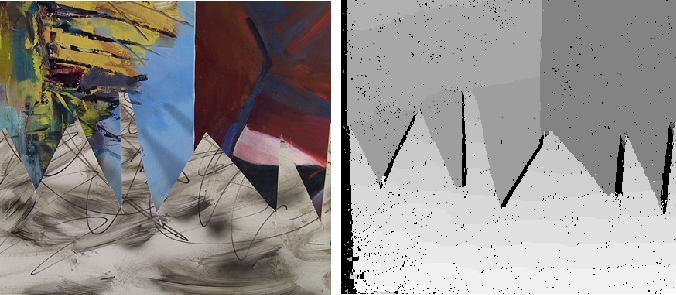
\includegraphics[width=0.8\textwidth]{images/overview_kolmogorov_graphcut}
  \caption{Ліве зображення та карта глибин,
           отримана за допомогою знаходження мінімального розрізу графу
           (зображення взяті зі статті \cite{overview:kolmogorov:graphcut})}
  \label{fig:overview:kolmogorov:graphcut}
\end{figure}

Для більш швидкої глобальної оптимізації
виконують сегментацію одного із зображень стереопари.
На пікселі в одному сегменті накладаютсья обмеження на зсуви так,
що при глобальній оптимізації оновлюється декілька змінних одразу
\cite{overview:ferg:graphcut}.

\section{Алгоритм дифузії}

Будується граф-решітка та мінімізується енергія \ref{eq:overview:energy}
шляхом розв'язання двоїстої задачі \cite{overview:savchynskyy:diffusion}.
Докладніше алгоритм описано в наступному розділі.

\section{Постановка задачі}

Виходячи з аналізу статей, запишемо постановку задачі,
яка буде розв'язана в наступних розділах.

Задане ліве півтонове зображення $L : T \to C$
та праве півтонове зображення $R : T \to C$
де
$T = \left\{
    \left( x, y \right) \; \middle| \; 1 \le x \le w, q \le y \le h
\right\}$~---~множина координат пікселів зображення,
$w$~---~ширина зображення (кількість пікселів на зображенні по горизонталі),
$h$~---~висота зображення (кількість пікселів на зображенні по вертикалі),
$C = \left\{ 0, \dotsc, 255 \right\} $~---~множина інтенсивностей пікселів.
Таким чином,
$L \left(x, y \right)$~---~це інтенсивність пікселя лівого зображення
з координатою $x$ по горизонталі та координатою $y$ по вертикалі,
а $R \left( x, y \right)$~---~це інтенсивність пікселя правого зображення
з координатою $x$ по горизонталі та координатою $y$ по вертикалі.

Вважається, що $L$ і $R$~---~пара зображень нерухомої сцени,
що зняті однією й тією ж камерою.
При цьому, праве зображення $R$ було отримано при тому ж напрямку зйомки,
що й ліве зображення $L$, але при зсуві камери строго горизонтально праворуч.
Це означає,
що проекції об'єктів на зображення також зміщуються виключно горизонтально.
Будуємо таку модель, згідно якої об'єкти не перекриваються один одним.
В експериментах, що наведені в четвертому розділі дисертації, показано,
що це не сильно обмежує застосування алгоритму~---~на практиці його можна
використовувати й для об'єктів, які перекриваються.

Таким чином, рядок з вертикальною координатою $y$
на лівому зображенні $L$ відповідає
рядку з вертикальною координатою $y$ на правому зображенні $R$
(рис.~\ref{fig:one:line}).
За рахунок паралаксу горизонтальна координата $x$
кожного пікселя лівого зображення $\left( x, y \right) \in T$
зсувається вліво на величину $d \left(x, y \right) $
для отримання координати відповідного пікселя на правому зображенні
$\left( x - d \left(x, y \right), y \right)$.
Множина всіх можливих зсувів $d \left(x, y \right)$
горизонтальної координати $x$ пікселя $\left(x, y \right)$ дорівнює
$D = \left\{ 0, \dotsc, M \right\}$, де $M$~---~фіксований максимальний зсув.

\begin{figure}[h]
  \centering
  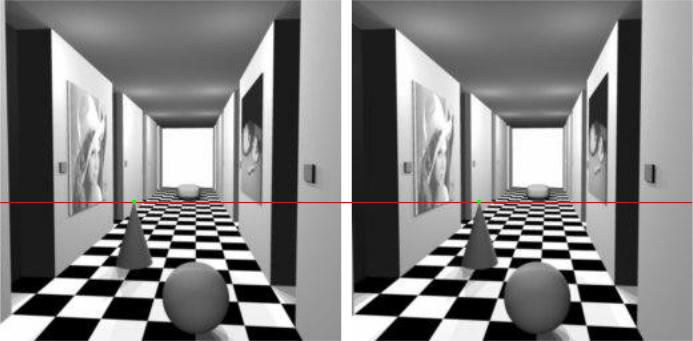
\includegraphics[width=0.8\textwidth]{images/one_line}
  \caption{Рядок з вертикальною координатою $y$
           на лівому зображенні $L$ відповідає
           рядку з вертикальною координатою $y$ на правому зображенні $L$
           (позначено червоною лінією).
           Зеленими точками позначена вершина конусу на двох зображеннях
           стереопари, яка лежить на одній горизонтальній лінії}
  \label{fig:one:line}
\end{figure}

Розглянемо задачу стереобачення в двовимірному світі,
де точки простору описуються двома невідомими координатами
$ \left( x, z \right) $ (рис.~\ref{fig:geometry}).
Задача полягає в знаходженні координати $z$,
яка визначає висоту точок в просторі,
для всіх пікселів на одному з зображень,
знятих камерою.
$C_1$~---~точка фокусу камери в першому положенні.
Вважаємо, що в ній знаходиться початок координат.
$C_2$~---~точка фокусу камери після зсуву її по горизонталі на відстань $b$.
Двома горизонтальними лініями позначені плівки, або площини,
на яких формуються зображення.
$f$~---~фокусна відстань камери~---~відстань від точки фокуса камери до плівки.
$x_1$ та $x_2$ позначають відстані від центрів зображень до променів,
що йдуть від точкок фокуса камери в двох положеннях до точки в прострорі.

\begin{figure}[h]
  \centering
  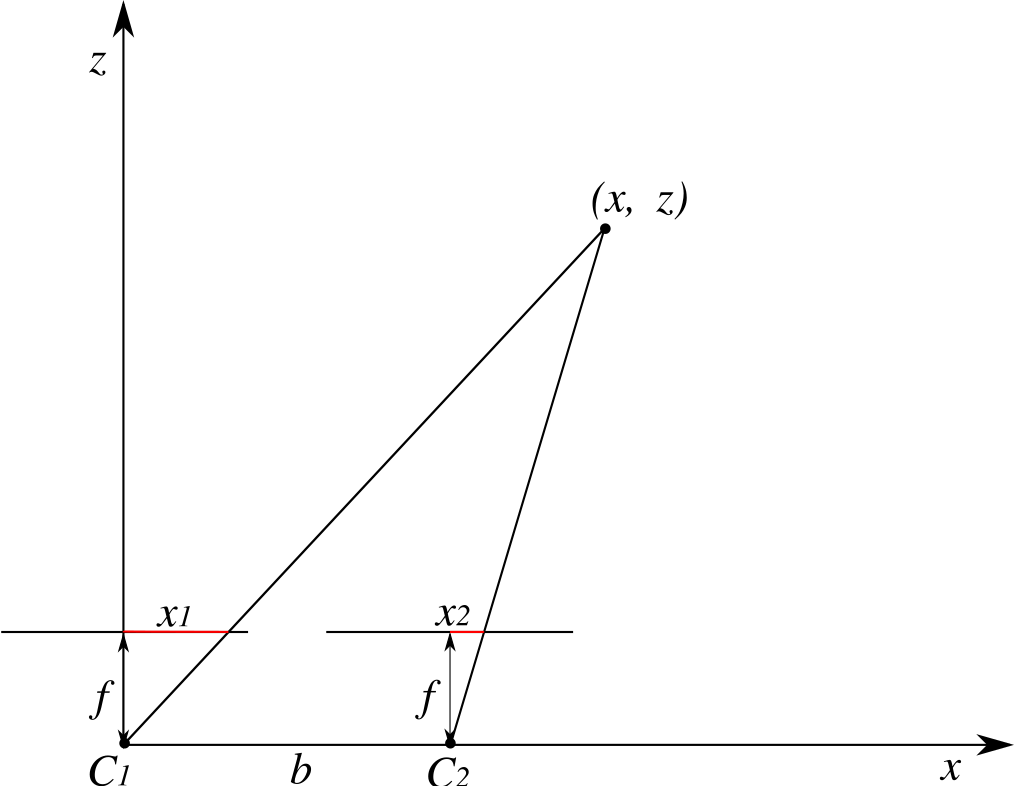
\includegraphics[width=0.8\textwidth]{images/2d_geometry}
  \caption{Одна точка простору, сфотографована камерою з двох положень}
  \label{fig:geometry}
\end{figure}

З подібності трикутників $\triangle BXC_1$ та $\triangle C_1 F_1 P_1$
(рис.~\ref{fig:triangles}) має місце співвідношення
\begin{equation}
    \frac{x}{z} = \frac{x_1}{f}.
\end{equation} \label{triangle:1}
З подібності трикутників $\triangle BXC_2$ та $\triangle C_2 F_2 P_2$
(рис.~\ref{fig:triangles}) має місце співвідношення
\begin{equation} \label{triangle:2}
    \frac{x - b}{z} = \frac{x_2}{f}.
\end{equation}

\begin{figure}[h]
  \centering
  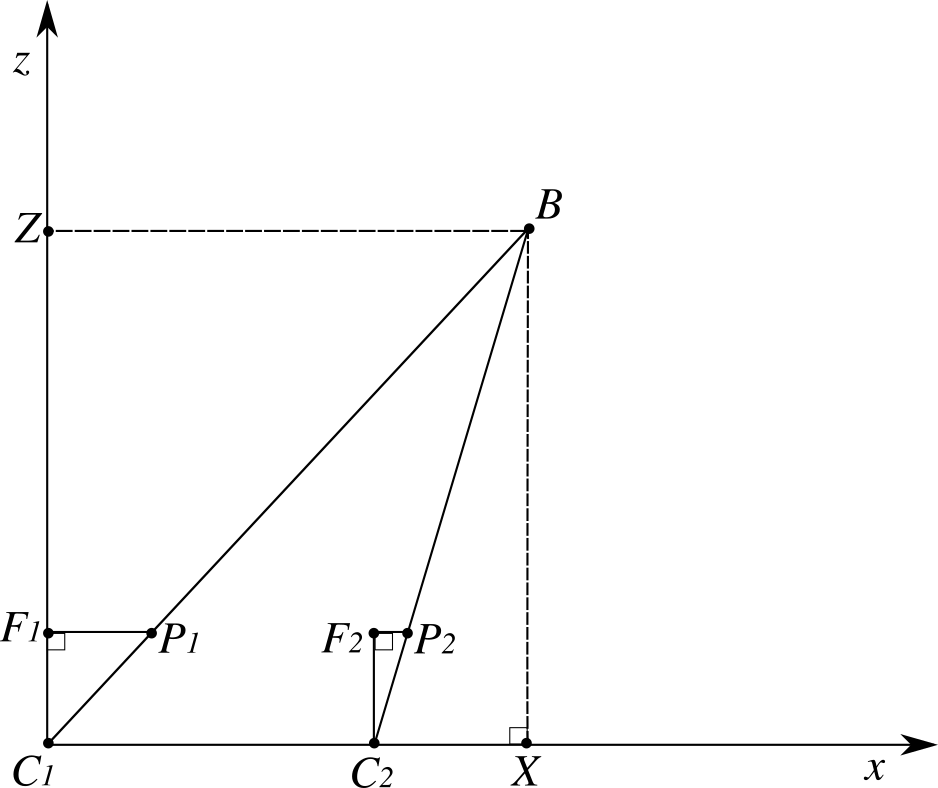
\includegraphics[width=0.8\textwidth]{images/2d_triangles}
  \caption{Подібні трикутники}
  \label{fig:triangles}
\end{figure}

Віднімемо співвідношення \eqref{triangle:2} від співвідношення
\eqref{triangle:1}
\begin{equation*}
    \frac{b}{z} = \frac{x_1 - x_2}{f},
\end{equation*}
звідки шукане значення координати $z$ дорівнює
\begin{equation*}
    z = \frac{b \cdot f}{x_1 - x_2} = \frac{b \cdot f}{d}.
\end{equation*}
Таким чином, щоб знайти положення точки в просторі,
необхідно знайти значення паралаксу $d$,
а також знати фокусну відстань камери $f$ та відстань,
на яку камера була зсунута по горизонталі $b$.

Далі розглядається задача пошуку значення паралаксу для всіх пікселів
лівого зображення $L$, тобто задача пошук карти глибин.

Будується $\left| T \right|$-дольний граф-решітка,
де кожній долі відповідає один піксель (рис.~\ref{fig:grid:graph:pixels}).
Будемо називати долі графу об'єктами.

\begin{figure}[h]
  \centering
  \includegraphics[width=0.6\textwidth]{images/grid_graph_pixels}
  \caption{$\left|T \right|$-дольний граф-решітка.
           Об'єкти (долі) позначені квадратами.
           Об'єкти, що поєднані лініями, є сусідніми}
  \label{fig:grid:graph:pixels}
\end{figure}


Кожен об'єкт $\left(y, x \right) \in T$ має $\left| D \right| $ вершин
$ \left( x, y, d \right)$,
які відповідають всім можливим зсувам $d \in D$ пікселя $\left(x, y \right)$
(рис.~\ref{fig:object:vertices}).
Значення зсувів $d \in D$ будемо називати мітками.

\begin{figure}[h]
  \centering
  \includegraphics[width=0.8\textwidth]{images/object_with_vertices}
  \caption{Об'єкт (позначений прямокутником) має $\left| D \right|$ вершин
           (позначені кружечками)}
  \label{fig:object:vertices}
\end{figure}

На кожну вершину $\left(x, y, d \right), \, d \in D$ в кожній долі графу
$\left(x, y \right) \in T$
накладається штраф за невідповідність інтенсивностей відповідних пикселів
\begin{equation*}
    f_{\left(x, y \right)} \left(d \right) =
    f \left(
        L \left(x, y\right),
        R \left(x - d, y \right)
    \right).
\end{equation*}
В цій роботі буде використовуватися наступний штраф для вершин
\begin{equation*}
    f_{\left(x, y \right)} \left( d \right) =
        \left| L \left(x, y \right) - R \left( x - d, y \right) \right|,
\end{equation*}
тобто модуль різниці інтенсивностей відповідних пікселів на двох зображеннях.

Кожен об'єкт графу має не більше чотирьох сусідніх об'єктів: верхній, правий,
нижній і лівий.
Об'єкти, що відповідають пікселям на границях зображення, мають по три сусіда,
а об'єкти, що відповідають кутовим пікселям,~---~по два.
Нехай $\mathcal{N} \left( x, y \right) $~---~множина всіх
сусідніх об'єктів для об'єкта $\left( x, y \right)$.
Всі вершини кожного об'єкту поєднані дужками з усіма
вершинами в сусідніх об'єктах (рис.~\ref{fig:neighbors}).

\begin{figure}[h]
  \centering
  \includegraphics[width=0.8\textwidth]{images/neighbors}
  \caption{Сусідні об'єкти до об'єкта $\left(x, y \right)$.
           Вершини в об'єктах позначені окружностями,
           всередині яких зазначені штрафи за вибір міток.
           Задля наочності дужки показані лише для вершини з міткою $d = 1$}
  \label{fig:neighbors}
\end{figure}

На дужку між вершиною з міткою $d \in D$ в об'єкті $\left(x, y \right)$
і вершиною з міткою $d' \in D$ в об'єкті $\left(x', y' \right)$
накладається штраф за невідповідність обраних зсувів в сусідніх об'єктах
$g_{\left(x, y \right), \left(x', y' \right)} \left(d, d' \right)$
(рис.~\ref{fig:neighbor:edge:weights}).
В цій роботі буде використовуватися наступний штраф для дужок
\begin{equation*}
    g_{\left(x, y \right), \left(x', y' \right)} \left(d, d' \right) =
        \alpha \cdot \left| d - d' \right|,
\end{equation*}
тобто модуль різниці обраних зсувів у двох сусідніх об'єктах,
де $\alpha$~---~коефіцієнт згладжування.
Множину всіх сусідніх об'єктів позначимо через $\mathcal{N}$.

\begin{figure}[h]
  \centering
  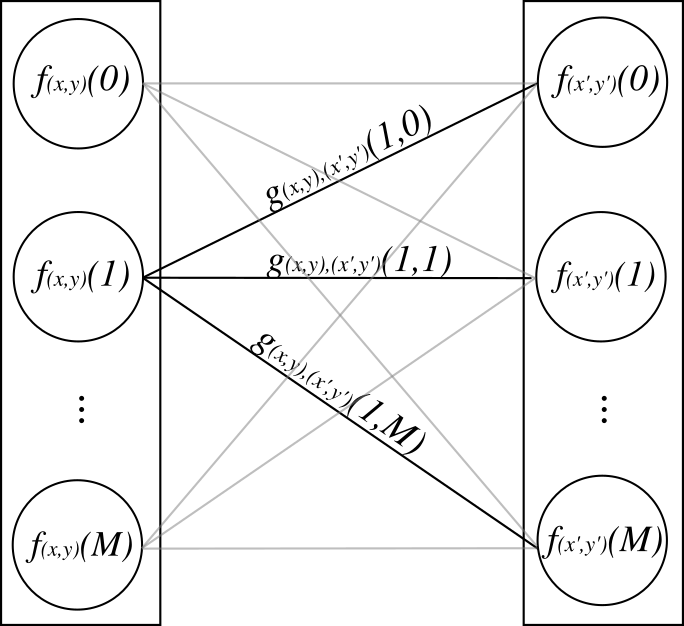
\includegraphics[width=0.6\textwidth]{images/neighbor_edge_weights}
  \caption{Ваги дужок, що йдуть від вершини з міткою $d = 1$ в об'єкті
           $\left(x, y \right)$ до всіх вершин в сусідньому об'єкті
           $\left(x', y' \right) \in \mathcal{N}\left(x, y \right)$.
           Ваги інших дужок записуються аналогічно}
  \label{fig:neighbor:edge:weights}
\end{figure}

Відображення $\pmb{d} : T \rightarrow D$ назвемо розміткою.
Кожному пікселю зображення (кожному об'єкту графу)
воно ставить у відповідність мітку,
тобто обирає одну й тільки одну вершину в кожному об'єкті
(рис.~\ref{fig:labeling}).
Задача полягає в такому виборі розмітки $\pmb{d} \in D^T$,
яка мінімізує штрафну функцію
\begin{equation} \label{eq:overview:penalty}
\begin{gathered}
    E \left( \pmb{d} \right)
    = \sum \limits_{\left(x, y \right) \in T}
        f_{\left(x, y \right)} \left(d \left(x, y \right) \right) + \\
    + \sum \limits_{\left(\left(x, y \right), \left(x', y'\right) \right) \in \mathcal{N}}
        g_{\left(x, y \right), \left(x', y' \right)} \left(
            d \left( x, y \right), d \left( x', y' \right)
        \right).
\end{gathered}
\end{equation}

\begin{figure}[h]
  \centering
  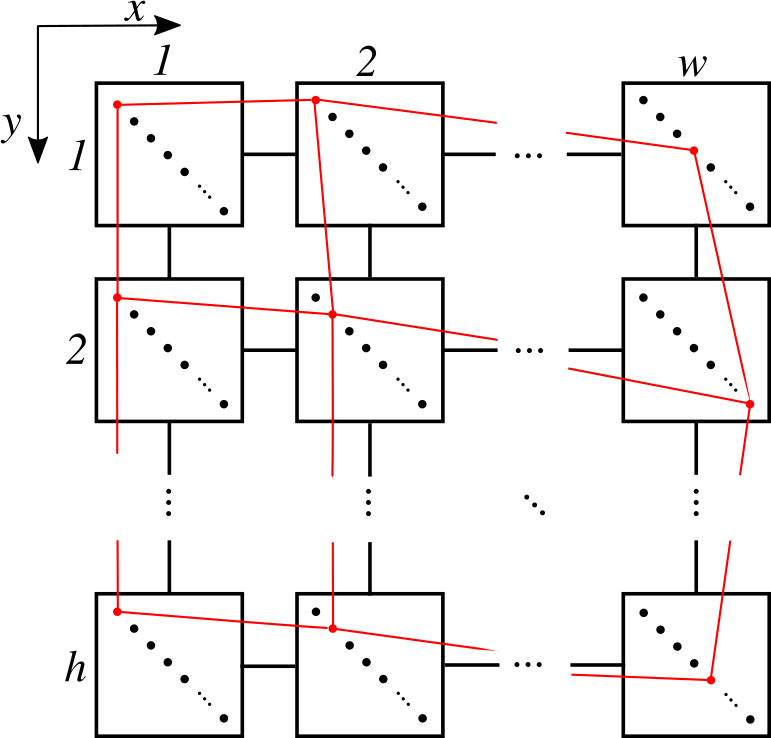
\includegraphics[width=0.6\textwidth]{images/labeling}
  \caption{Візуалізація розмітки.
           Об'єкти позначені квадратами.
           Об'єкти, поєднані чорними лініями є сусідніми.
           Вершини в об'єктах позначені кружечками.
           Розмітка позначена червоним}
  \label{fig:labeling}
\end{figure}

\section*{Висновки до розділу 1}
\addcontentsline{toc}{section}{Висновки до розділу 1}

Проведено огляд алгоритмів,
які використовуються для розв'язання задачі стереобачення.
Поставлена задача,
розв'язання якої наведено в наступних роздiлах дисертації.

Наведена постановка задачі є природною,
адже враховує залежність проекції об'єктів з простору
в одному пікселі від проекцій об'єктів в інших пікселях,
наприклад, якщо один гладкий об'єкт зайняв більше одного рядка зображення.
В постановці задачі,
що використовується для
розв'язання задачі стереобачення методом динамічного пограмування,
залежності між рядками немає, тобто вважається,
що об'єкти, спроектовані в різні рядки зображення, є незалежними,
що на практиці не відповідає дійсності.
